\documentclass[a4paper,11pt,answers]{exam}

\usepackage[linesnumbered,ruled,vlined]{algorithm2e}
\usepackage{amsfonts,amsmath,amssymb,amsthm}
\usepackage[english]{babel}
\usepackage{cancel}
\usepackage{caption}
\usepackage{enumitem}
\usepackage[a4paper,left=1cm,right=1cm,top=2.5cm,bottom=2.5cm]{geometry}
\usepackage{graphicx}
\usepackage{hyperref}
\usepackage{float}
\usepackage[bb=boondox]{mathalpha,mathtools}
\usepackage{nicematrix}
\usepackage{dsfont}
\usepackage{xpatch}
\usepackage{graphicx}
\usepackage{subcaption}
\xpatchcmd{\questions}
{question@\arabic{question}}
{question@\arabic{section}@\arabic{question}}
{}{}
\qformat{\textbf{\thequestion.}\quad}


\newtheorem{theorem}{Theorem}

\title{LINMA2450 --- Project Part 1 \\ Combinatorial Optimization}
\author{Brieuc Dallemagne \texttt{77122100} \and Alois Tavier \texttt{58242100}}
\date{}

\begin{document}
\renewcommand{\thesection}{\Alph{section}}
\renewcommand{\solutiontitle}{}
\allowdisplaybreaks{}
\maketitle

\section*{Problem 1 --- Optimal Boards Cutting}

\begin{parts}
    \part \textbf{(1.1) Knapsack.}
    \begin{solutionorbox}
    A cutting pattern is feasible if the total sum of the lengths $l_j$ of the pieces cut from a large board does not exceed the board length \(L\). 
    So we can express $X$, the set of all feasible patterns, as a knapsack-type constraint:
    \[
    \sum_{j=1}^{n} l_j\, x_{j} \leq L, \quad x_{j} \in \mathbb{N}, \quad x \in X.
    \]
    We can formulate this as follow: \begin{equation*}
        X=\bigg\{ x\in \mathbb{N}^n :  \sum_{j=1}^{n} l_j\, x_{j} \leq L \bigg\}
    \end{equation*}
    \end{solutionorbox}

    \part \textbf{(1.2) Model P1.}
    \begin{solutionorbox}

    Let \(X\) denote the set of feasible cutting patterns \(x \in P\), where \(x_j\) is the number of items of type \(j\) in pattern \(x\) and \(y_{x} \in \mathbb{N}\) represents the number of boards cut according to pattern \(x\).
    \[
    \begin{aligned}
    \text{(P1)}\quad 
    \underset{y_x \in \mathbb{N}}{\min}\;& \sum_{x\in X} y_x\\
    \text{s.t.}\;& \sum_{x\in X} x_{j}\,y_x \;\ge\; d_j, && j=1,\ldots,n
    \end{aligned}
    \]
    or in matrix form with $T:=|X|$, $y\in \mathbb{N}^{T}$,  $A\in \mathbb{N}^{ n\times T}$ such that $a_{jt}=x^t_j$ and $d =  \
    [d_1, \cdots, d_n]$ we obtain:
    \[
    \begin{aligned}
    \text{(P1)}\quad 
    \underset{y \in \mathbb{N}^T}{\min}\;& y^\top \mathds{1} \\
    \text{s.t.}\;& A \cdot y \;\ge\; d, && x^t \in X.
    \end{aligned}
    \]

    \end{solutionorbox}

    \part \textbf{(1.3) Size and Tractability.}
    \begin{solutionorbox}
    Let's take an example where $L=n$ and $l_j=1$ for $j=1, \dots, n$:\\
    The constraints is the following:
    \begin{equation*}
        X = \bigg\{x \in \mathbb{N}^n \Big|  \sum_{j=1}^n x_j \leq n\bigg\}
    \end{equation*}
    Every binary vector $x\in \{0,1\}^n$ is a valid solution but $|\{0,1\}^n|$ is smaller than $|X|$ because this doesn't include the cases where $x_j> 1$. Let's construct a lower bound:
    \begin{equation*}
        |X| \geq |\{0,1\}^n| = 2^n
    \end{equation*}
    We know that the number of variable in the model is $T=|X|$ and that the size of $X$ can grow exponentially in certain cases with the number of customer's demands. This exponential growth in feasible patterns makes enumeration computationally in-tractable, confirming that the cutting stock problem is NP-hard.
    \end{solutionorbox}

    \part \textbf{(2.1) Implementation of greedy heuristic.}
    \begin{solutionorbox}
    implementation : see notebook
    
    At each step the heuristic selects, among all items that still fit in the remaining capacity,
    the one with the largest length (ties broken by highest residual demand), and inserts it once.
    This is repeated until no further item fits.
    \end{solutionorbox}
    \part \textbf{(2.2) proof.}
    \begin{solutionorbox}
    Let's define \[z^1 = \sum_{x\in \tilde{X}}\Bar{y}_x \quad \text{s.t.} \; \; \sum_{x\in \tilde{X}}x_j\Bar{y}_x \geq d_j, \; \; j=1, \dots, n\]
    a solution of the problem $P_1$ with $\tilde{X}$.\\
    It is also a solution of $P_1$ with $X$ because it is admissible, i.e. respect the problem's constraints:
    \[\sum_{x\in X}x_j y_x = \sum_{x\in \tilde{X}}x_j \Bar{y}_x + \sum_{x\in X\backslash\tilde{X}}x_j\cdot 0 = \sum_{x\in \tilde{X}}x_j \Bar{y}_x \geq d_j \quad j=1, \dots, n\]
    So we have a primal solution of $P_1$ with $X$ taking the solution $\Bar{y}$ of $P_1$ with $\tilde{X}$:
    \[
    \begin{cases}
        y_x=\Bar{y}_x \;\; \text{if} \;\; x\in \tilde{X}\\
        y_x=0 \quad \text{if} \;\; x\in X\backslash \tilde{X}
    \end{cases}
    \]
    This gives an uperbound to the problem optimal solution of the problem $P_1$ with $X$ as $z^1 \geq z^*$.
    \end{solutionorbox}
    \part \textbf{(2.3) Algorithm.}
    \begin{solutionorbox}
    At iteration $k$, solving $P_1$ with the current set of patterns $\tilde X^k$ gives an optimal
    solution $y^k$.  
    From this we compute the residual demand of each item
    \[
        r_j^k \;=\; d_j - \sum_{x\in \tilde X^k} x_j\,y_x^k ,\qquad j=1,\dots,n.
    \]
    The information stored in $s$ is therefore $s=(y^k,r^k)$.

    The procedure \textsc{NewPattern}$(s)$ constructs a new pattern by solving a knapsack problem
    with capacity $L$, item lengths $l_j$ and profits $r_j^k$ using a greedy rule:
    \begin{enumerate}
        \item sort the items $j$ in non-increasing order of the ratio $r_j^k/l_j$;
        \item starting from the first item in this order, insert as many copies as possible while
              respecting $\sum_j l_j x_j \le L$;
        \item continue with the next items in the list until no further piece fits.
    \end{enumerate}
    The resulting vector $x^{\text{new}}$ satisfies $\sum_j l_j x_j^{\text{new}} \le L$. It is a feasible cutting pattern and we set $\textsc{NewPattern}(s)=x^{\text{new}}$.

    Since the profits are proportional to the residual demands, the pattern focuses on items with
    large remaining demand. Adding such a pattern to $\tilde X^k$ is therefore likely to allow
    $P_1$ to cover the demands with fewer boards and then to improve the primal upper bound.
    \end{solutionorbox}

    \part \textbf{(3) Implementation and comparison.}
    \begin{solutionorbox}
    Implementation : see notebook
    
    We solved all instances using the HiGHS solver.  
    For every provided instance, the primal bound obtained with our restricted pattern set coincides with what we found when we calculate the optimal value in the files that we created with BPPlib.  
    CPU times were never that big but we put our time limit at 20 seconds for those instances. 
    \smallskip

    Here we made a plot to see the complexity of the solver:
    
    \begin{center}
    \includegraphics[width=0.85\textwidth]{../csp_solving_time.png}
    \end{center}
    
    As we could except from Q1.3, the plot shows that the solving time grows exponentially with the instance size.\\

    Here is the result we got from the exemple of assignement:
    Objective (nbr of long boards used) = 4.0   Status = OPTIMAL   Time = 0.022 s
    \end{solutionorbox}
\clearpage
    
\end{parts}

\section*{Problem 2 --- Optimal Delivery Assignment}

\begin{parts}
    \part\textbf{(1.1) Model — Optimal Delivery Assignment}
    \begin{solutionorbox}
 
    First we precompute
    \[
    c_{ij}=\operatorname{dist}_G(i,j)
    \quad\text{(shortest-path length from }i\in D\text{ to }j\in C\text{; set }c_{ij}=+\infty\text{ if unreachable).}
    \]
    
    We create binary variables $x_{ij}$ s.t for each $i\in D$, $j\in C$,
    \[
    x_{ij}\in\{0,1\}\quad\text{equals 1 if client }j\text{ is served by warehouse }i.
    \]
    
    the we create our MILP formulation as.
    \[
    \min_{x}\ \sum_{i\in D}\sum_{j\in C} c_{ij}\,x_{ij}
    \]
    \[
    \sum_{i\in D} x_{ij}=1 \quad \forall\, j\in C \qquad\text{(each client is assigned)}
    \]
    To fit the model used by the Hungarian method we can add a last constraint:
    \[
    \sum_{j\in C} x_{ij}\le 1 \quad \forall\, i\in D \qquad\text{(at most one client per warehouse)}
    \]
    \[
    x_{ij}\in\{0,1\}.
    \]
    
    \end{solutionorbox}
    
    \part\textbf{(1.2) The Hungarian Method}
    \begin{solutionorbox}
    The Hungarian method is a combinatorial optimization technique used to solve the
    assignment problem for 2 sets of the same size (finding a minimum-cost one-to-one matching between two sets).

    Main idea: The method transforms the cost matrix step by step:
    \begin{enumerate}
    \item Subtract the smallest element in each row and column so that every row and column contains at least one zero.
    \item Select a maximum set of independent zeros (one per row and column).
    \item If all rows or columns are covered, the corresponding assignment is optimal.
    Otherwise, adjust the uncovered elements and repeat until a complete matching is obtained.
    \end{enumerate}

    In our case the matrix might be rectangular. (when $|D|> |C|$) So, we added dummy rows with a cost of zero to obtain a square matrix.

    \textbf{Complexity.} The algorithm runs in polynomial time \(O(n^3)\) and guarantees an optimal
    solution for any finite cost matrix.
    \end{solutionorbox}
    
    \part\textbf{(1.3) Optimality and Tractability}
    \begin{solutionorbox}
    The Hungarian method always finds an optimal solution because it is based on the
    duality principle of linear programming.
    At each iteration, the algorithm maintains feasible dual variables (row and column reductions)
    and ensures complementary slackness with respect to zero-cost entries.
    
    \smallskip
    When all tasks are assigned, the primal (assignment) and dual (reduction) conditions are both
    satisfied, proving optimality.
    
    \smallskip
    \textbf{Tractability.} The assignment problem is efficiently solvable in polynomial time.
    Its linear relaxation is integral since the constraint matrix is totally unimodular, ensuring that
    the optimal solution of the relaxed problem is also integer.
    \end{solutionorbox}



    \part \textbf{(2.1) implementation MILP.}
    \begin{solutionorbox}
    see notebook
    \end{solutionorbox}

    \part \textbf{(2.2) implementation Hungarian Method.}
    \begin{solutionorbox}
    see notebook
    \end{solutionorbox}

    \part \textbf{(2.3) Implementation and Comparison.}
    \begin{solutionorbox}

    \begin{center}
    \begin{minipage}{0.48\textwidth}
        \centering
        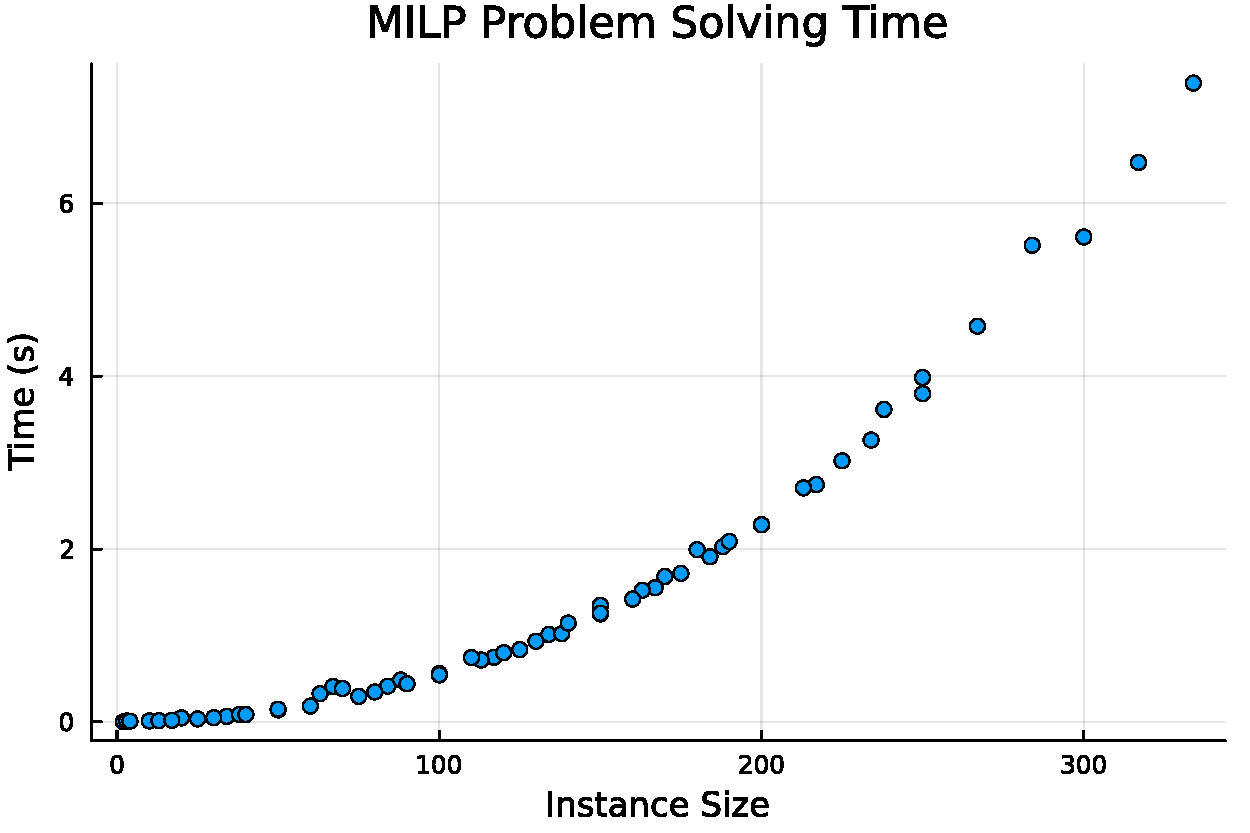
\includegraphics[width=1.1\textwidth]{../MILP_solving_time.pdf}
    \end{minipage}
    \hfill
    \begin{minipage}{0.5\textwidth}
        \centering
        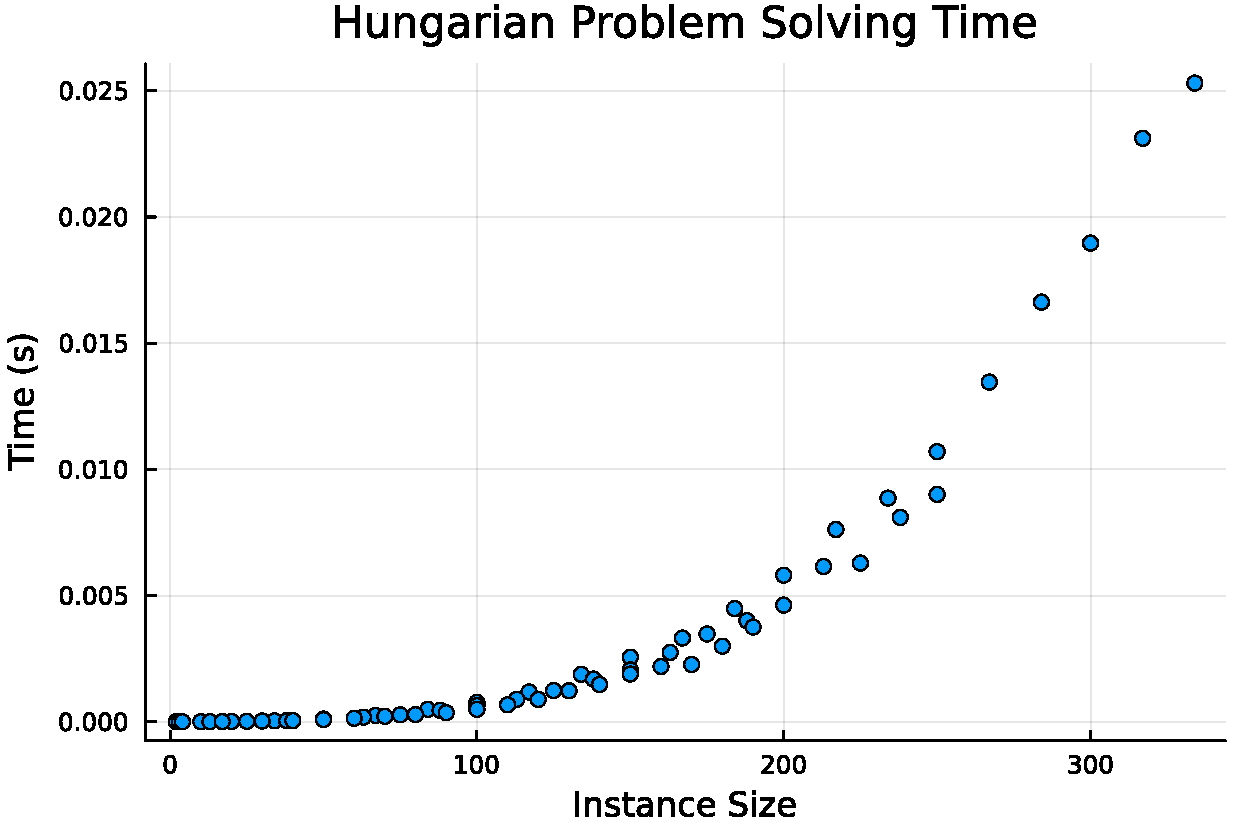
\includegraphics[width=1.05\textwidth]{../Hungarian_solving_time.pdf}
    \end{minipage}
    \end{center}
    Both methods show increasing runtimes as the instance size grows. The Hungarian method exhibits a visible rise for larger instances, but its absolute solving time remains in the millisecond range. The MILP solver, however, grows far more rapidly, reaching several seconds and displaying clear non-polynomial scaling. Even though both curves increase, the Hungarian method remains vastly faster across all instances. 
    \end{solutionorbox}

\end{parts}

\begin{thebibliography}{9}

\bibitem{wiki_assignment}
Wikipedia contributors, 
\emph{Assignment problem}, 
\textit{Wikipedia, The Free Encyclopedia}, 
available at: \url{https://en.wikipedia.org/wiki/Assignment_problem}, 
accessed November 2025.

\bibitem{byjus_assignment}
BYJU’S, 
\emph{Assignment Problem – Definition, Methods, and Solved Examples}, 
available at: \url{https://byjus.com/maths/hungarian-method/}, 
accessed November 2025.

\bibitem{geeksforgeeks_hungarian}
GeeksforGeeks, 
\emph{Hungarian Algorithm for Assignment Problem (Set 1 – Introduction)}, 
available at: \url{https://www.geeksforgeeks.org/dsa/hungarian-algorithm-assignment-problem-set-1-introduction/}, 
accessed November 2025.

\end{thebibliography}



\end{document}